\documentclass[]{article}
\usepackage{lmodern}
\usepackage{amssymb,amsmath}
\usepackage{ifxetex,ifluatex}
\usepackage{fixltx2e} % provides \textsubscript
\ifnum 0\ifxetex 1\fi\ifluatex 1\fi=0 % if pdftex
  \usepackage[T1]{fontenc}
  \usepackage[utf8]{inputenc}
\else % if luatex or xelatex
  \ifxetex
    \usepackage{mathspec}
  \else
    \usepackage{fontspec}
  \fi
  \defaultfontfeatures{Ligatures=TeX,Scale=MatchLowercase}
\fi
% use upquote if available, for straight quotes in verbatim environments
\IfFileExists{upquote.sty}{\usepackage{upquote}}{}
% use microtype if available
\IfFileExists{microtype.sty}{%
\usepackage{microtype}
\UseMicrotypeSet[protrusion]{basicmath} % disable protrusion for tt fonts
}{}
\usepackage[margin=1in]{geometry}
\usepackage{hyperref}
\hypersetup{unicode=true,
            pdftitle={hierarchical\_summary},
            pdfauthor={Ben Smith},
            pdfborder={0 0 0},
            breaklinks=true}
\urlstyle{same}  % don't use monospace font for urls
\usepackage{longtable,booktabs}
\usepackage{graphicx,grffile}
\makeatletter
\def\maxwidth{\ifdim\Gin@nat@width>\linewidth\linewidth\else\Gin@nat@width\fi}
\def\maxheight{\ifdim\Gin@nat@height>\textheight\textheight\else\Gin@nat@height\fi}
\makeatother
% Scale images if necessary, so that they will not overflow the page
% margins by default, and it is still possible to overwrite the defaults
% using explicit options in \includegraphics[width, height, ...]{}
\setkeys{Gin}{width=\maxwidth,height=\maxheight,keepaspectratio}
\IfFileExists{parskip.sty}{%
\usepackage{parskip}
}{% else
\setlength{\parindent}{0pt}
\setlength{\parskip}{6pt plus 2pt minus 1pt}
}
\setlength{\emergencystretch}{3em}  % prevent overfull lines
\providecommand{\tightlist}{%
  \setlength{\itemsep}{0pt}\setlength{\parskip}{0pt}}
\setcounter{secnumdepth}{0}
% Redefines (sub)paragraphs to behave more like sections
\ifx\paragraph\undefined\else
\let\oldparagraph\paragraph
\renewcommand{\paragraph}[1]{\oldparagraph{#1}\mbox{}}
\fi
\ifx\subparagraph\undefined\else
\let\oldsubparagraph\subparagraph
\renewcommand{\subparagraph}[1]{\oldsubparagraph{#1}\mbox{}}
\fi

%%% Use protect on footnotes to avoid problems with footnotes in titles
\let\rmarkdownfootnote\footnote%
\def\footnote{\protect\rmarkdownfootnote}

%%% Change title format to be more compact
\usepackage{titling}

% Create subtitle command for use in maketitle
\newcommand{\subtitle}[1]{
  \posttitle{
    \begin{center}\large#1\end{center}
    }
}

\setlength{\droptitle}{-2em}
  \title{hierarchical\_summary}
  \pretitle{\vspace{\droptitle}\centering\huge}
  \posttitle{\par}
  \author{Ben Smith}
  \preauthor{\centering\large\emph}
  \postauthor{\par}
  \predate{\centering\large\emph}
  \postdate{\par}
  \date{7/15/2018}


\begin{document}
\maketitle

\subsection{A two-level hierarchical model of behavioral analysis of all
subjects across the
task.}\label{a-two-level-hierarchical-model-of-behavioral-analysis-of-all-subjects-across-the-task.}

I analyzed a number of subjects and found that across the group, meth
users had lower learning rates than non-meth users.

\begin{verbatim}
## [1] "compiling.."
\end{verbatim}

\begin{verbatim}
## [1] "compiling.."
\end{verbatim}

\begin{verbatim}
## [1] 4
## [1] 8
## [1] 12
## [1] 17
## [1] 21
## [1] 25
## [1] 29
## [1] 33
## [1] 38
## [1] 42
## [1] 46
## [1] 50
## [1] 54
## [1] 58
## [1] 62
## [1] 67
## [1] 71
## [1] 75
## [1] 79
## [1] 83
## [1] 88
## [1] 92
## [1] 96
## [1] 100
\end{verbatim}

\begin{verbatim}
## pdf 
##   2
\end{verbatim}

This is derived from raw\_data\_all\_runs\_flat\_v2.R.

\begin{verbatim}
## [1] 0.000807 2.475415
\end{verbatim}

\begin{verbatim}
## 
##      FALSE       TRUE 
## 0.01669164 0.98330836
\end{verbatim}

\begin{verbatim}
## [1] -2.305174 -0.113698
\end{verbatim}

\begin{verbatim}
## [1] -0.212635  0.284750
\end{verbatim}

\begin{verbatim}
## [1] -1.470363  0.644386
\end{verbatim}

\begin{verbatim}
## [1] -1.767819  0.319997
\end{verbatim}

\includegraphics{hierarchical_summary_2018_april_results_files/figure-latex/flat_behavioral_analysis-1.pdf}

\begin{verbatim}
## [1]   24 1001    6
\end{verbatim}

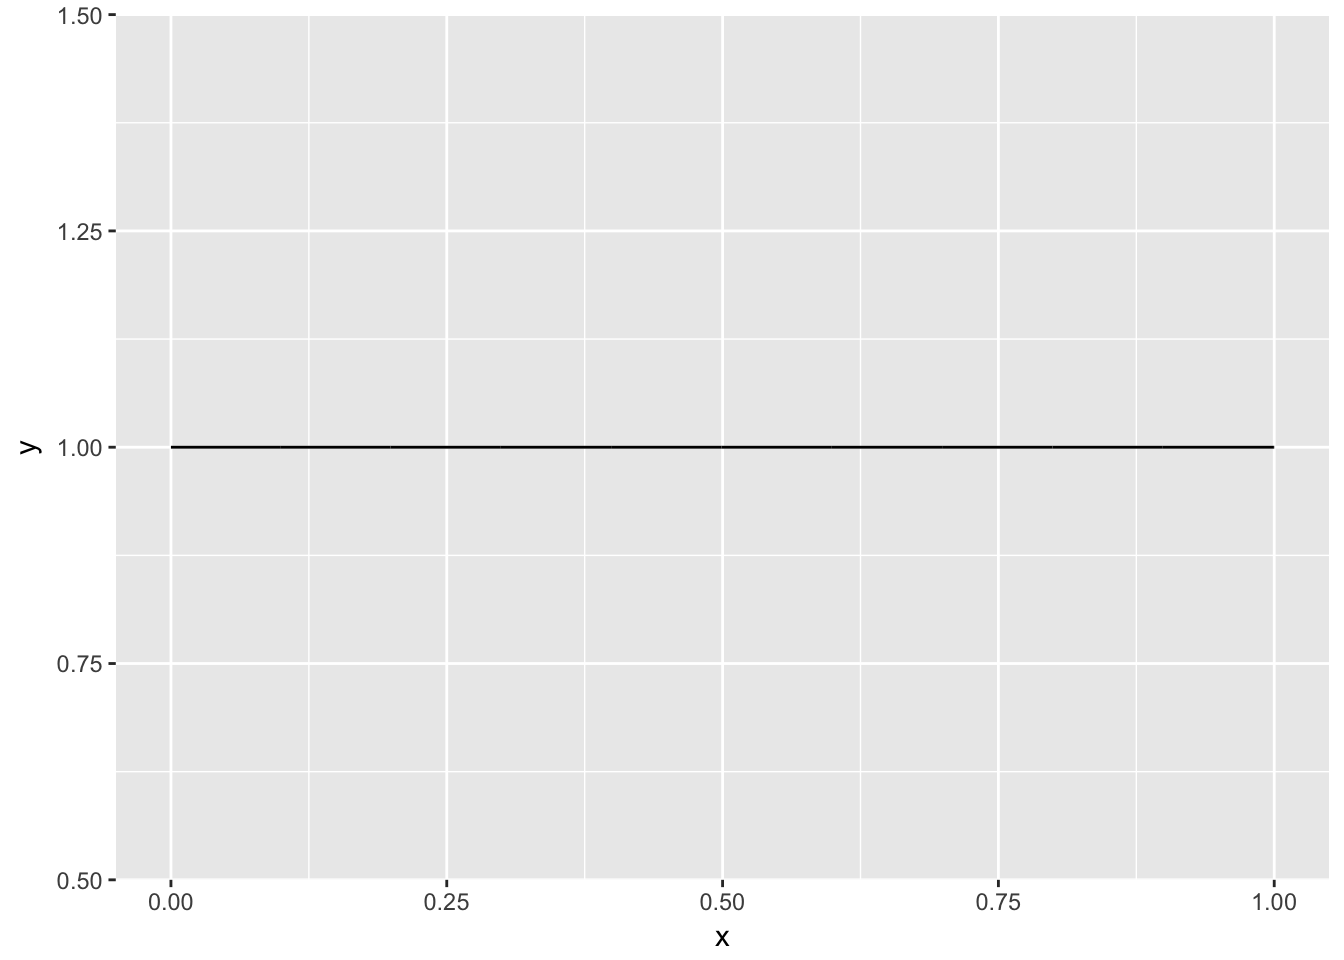
\includegraphics{hierarchical_summary_2018_april_results_files/figure-latex/unnamed-chunk-1-1.pdf}

\subsection{Parameters}\label{parameters}

Here is the HDI for each of the parameters for this model.

The learning rate difference between meth-using subjects and
non-meth-using subjects was significant.

\begin{longtable}[]{@{}llll@{}}
\toprule
& alpha\_mu & thresh\_mu & tau\_mu\tabularnewline
\midrule
\endhead
sr\_diff & {[}-0.601, 1.701{]} & {[}-0.231, 0.208{]} & {[}8.07e-04,
2.475{]}\tabularnewline
meth\_diff & {[}-2.305, -0.114{]} & {[}-0.213, 0.285{]} & {[}-1.470,
0.644{]}\tabularnewline
sr\_meth\_diff & {[}-1.768, 0.320{]} & {[}-0.246, 0.299{]} & {[}-0.616,
2.191{]}\tabularnewline
\bottomrule
\end{longtable}


\end{document}
